\chapter{相关理论与技术概述}
\label{chap:knowledge}

\section{Rust:依赖语言的程序设计}

Rust\pagescite{rust0} 是一门十分高效的编程语言, 其设计目的是在编译时提供强大的类型和内存安全保证,它将高级托管语言的强大功能和表达能力与类似c语言的无垃圾收集或底层运行时的效率相结合。编写操作系统可以利用Rust的许多特性来实现语言内、安全的操作系统设计,并使用crate (Rust的项目容器和翻译单元)实现源代码级模块化。而Cargo.toml包含源代码和依赖项清单。

\section{Riscv指令集}

RISC-V\pagescite{riscv0}指令集是基于精简指令集计算(RISC)原理建立的开放指令集架构(ISA),RISC-V是在指令集不断发展和成熟的基础上建立的全新指令。RISC-V指令集是开源的,由于设计简单,该指令集易于移植。Riscv的模块化设计和完整的开发工具链,使其拥有大量的开源实现和流片。

\section{异步的理解}
\begin{figure}[htb]
    \figureCapSet
    \centering
    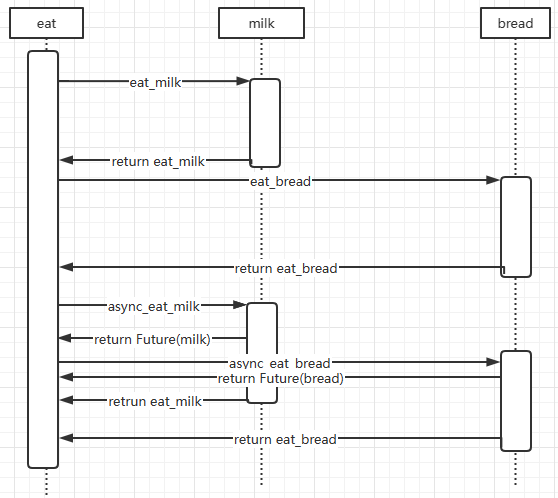
\includegraphics[scale=0.5]{figure/c2/breakfirstsequence.png}
    \caption{Breakfirst的同步和异步}
    \label{figure:c2breakfirstsequence}
\end{figure}

如\autoref{figure:c2breakfirstsequence}所示,这张序列图显示了一个eat函数的执行时序。该函数先执行了同步的eat\_milk和eat\_bread函数,又执行了async\_eat\_milk和async\_eat\_bread函数。先后两次同步和两次异步。

在同步调用的时候,函数是排队执行的,从牛奶到面包是依次进行,在牛奶喝完之前,不可以啃面包,事情只能一步一步完成,而完成的信号就是相应函数的返回。

在异步调用的时候,喝牛奶时,可以返回Futre,牛奶的工作会被置换到后台,然后掉起啃面包的行为,这个动作同样是异步的,换句话说,当面包的工作出现阻塞时,面包同样可以被置换到后台,让出资源。这样的工作使得相应函数可以更早地被执行,然后形成宏观上相应动作地并发执行,而无需在接收函数返回之前长时间的等待。
